%\begin{enumerate}[label=\arabic*.,ref=\theenumi]
\begin{enumerate}[label=\thesection.\arabic*.,ref=\thesection.\theenumi]
\numberwithin{equation}{enumi}
%2.1.1
%\item Consider the Magnitude Bode Plot and Phase Bode Plot \ref{fig:ee18btech11014_Bode} of Open-Loop Transfer Function of an Amplifier. Estimate the Open-Loop Transfer Function. (Assume $'A'$ as $'G'$ and $'\beta'$ as $'H'$)
%\begin{figure}[ht!]
%	\begin{center}
%		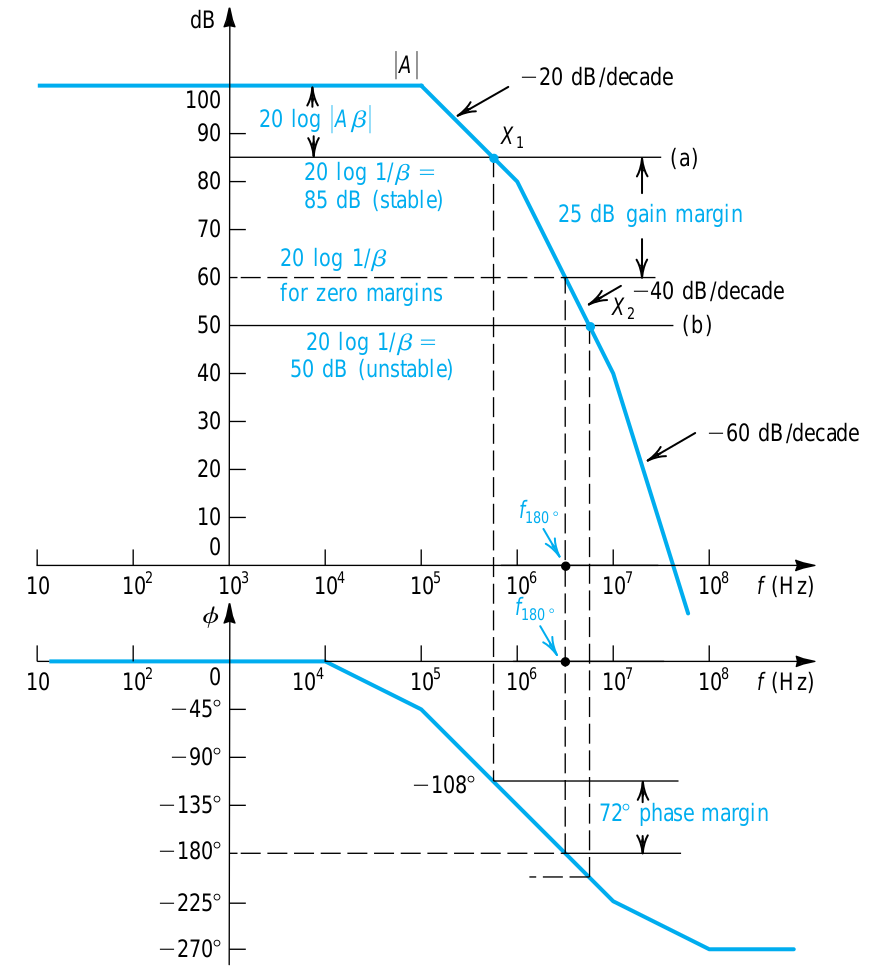
\includegraphics[width=\columnwidth]{./figs/ee18btech11014/ee18btech11014_figa.eps}
%	\end{center}
%	\caption{Magnitude and Phase Bode Plot}
%	\label{fig:ee18btech11014_Bode}
%\end{figure}\\
%\solution Let $G(f)$ be the Open-Loop Transfer Function,
%\begin{align}
%G(f) = 
%\begin{cases} 
%      100 & 0 < f < 10^{5} \\
%      200-20\log(f) & 10^{5} < f < 10^{6} \\
%      320-40\log(f) & 10^{6} < f < 10^{7} \\
%      460-60\log(f) & 10^{7} < f  \\
%\end{cases}
%\end{align}
%
%\begin{align}
%\nabla G(f) &= \dfrac{d(G(f))}{d(\log(f))} =
%\begin{cases} 
%        0 & 0 < f < 10^{5} \\
%      -20 & 10^{5} < f < 10^{6} \\
%      -40 & 10^{6} < f < 10^{7} \\
%      -60 & 10^{7} < f  \\ 
%\end{cases}
%\end{align}
%
%As we know that, \textbf{When a pole is encountered the slope always decreases by 20 dB/decade} and \textbf{When a zero is encountered the slope always increases by 20 dB/decade}. So, by observing Fig. \ref{fig:ee18btech11014_Bode} it can be concluded that we are having Poles at $f=10^{5} Hz, 10^{6} Hz, 10^{7} Hz$ and No Zeros.\\
%
%So, the Open-Loop Transfer Function $G(f)$ is
%\begin{align}
%\label{eq:ee18btech11014_G}
%	G(f) = \dfrac{10^{5}}{\left(1+j\frac{f}{10^{5}}\right)\left(1+j\frac{f}{10^{6}}\right)\left(1+j\frac{f}{10^{7}}\right)}
%\end{align}\\
%%-------------------------------------------------------------------------------------------------%
%%2.1.2
%\item Calculate the Phase of Open-Loop Transfer Function.\\
%\solution
%%
%\begin{multline}
%\label{eq:ee18btech11014_G_ang}
%\phi\brak{f} =
%\\
%-\sbrak{\tan ^{-1}\brak{\frac{f}{10^{5}}}+\tan ^{-1}\brak{\frac{f}{10^{6}}}+\tan ^{-1}\brak{\frac{f}{10^{7}}}}
%\end{multline}
%%-------------------------------------------------------------------------------------------------%
%%2.1.3
%\item Find the PM from  Fig. 	\ref{fig:ee18btech11014_Bode}, given that he feedback gain $H(f)$ is constant and given by 
%\begin{align}
%20 \log \brak{\frac{1}{H(f) }} &= 85 dB
%\\
%\text{or, } H(f) &= 5.623 \times 10^{-5}.
%\end{align}
%\\
%\solution From the figure, 
%\begin{align}
%\label{eq:ee18btech11014_G_f1}
%20 \log \abs{G(f_1)} &= 85 dB
%\\
%\implies 20 \log \abs{G(f_1)} & = 20 \log \brak{\frac{1}{H(f_1) }}
%\\
%\text{or, } \abs{G(f_1)H(f_1)} &= 1
%\end{align}
%and 
%\begin{align}
%\label{eq:ee18btech11014_f1}
%f_1 = 0.493 MHz, 
%\end{align}
%from \eqref{eq:ee18btech11014_G_f1} and \eqref{eq:ee18btech11014_G}.
%Also,
%%
%\begin{align}
%\because \phase{H(f)} &= 0, \forall f
%\\
%\phase{G(f_1)H(f_1)} &= \phase{G(f_1)} = -108 \degree
%\\
%\implies PM &= 180 \degree - 108 \degree = 72 \degree
%\end{align}
%using \eqref{eq:ee18btech11014_f1} in \eqref{eq:ee18btech11014_G_ang}.
%
%%-------------------------------------------------------------------------------------------------%
%\item Find the GM.
%\\
%\solution The crossover frequency $f_{\pi}$ is defined as 
%\begin{align}
%\phase{G\brak{f_{\pi}}H\brak{f_{\pi}}} &= 180 \degree
%\\
%\implies \phase{G\brak{f_{\pi}}} &= 180 \degree
%\\
%\implies f_{\pi} &= 3.34 MHz
%\end{align}
%by solving \eqref{eq:ee18btech11014_G_ang}.
%From Fig. \ref{fig:ee18btech11014_Bode}, 
%\begin{align}
%\label{eq:ee18btech11014_G_f1}
%20 \log \abs{G(f_\pi)} &= 60 dB
%\\
%\implies 20 \log \abs{G(f_\pi)} &-  20 \log \brak{\frac{1}{H(f_\pi) }}   
%\nonumber \\
%&= \brak{60 -85} dB
%\\
%\implies GM &= \abs{20 \log \abs{G(f_\pi)H(f_\pi) }} 
%\nonumber \\
%&= 25 dB
%\end{align}
%%

%-------------------------------------------------------------------------------------------------%
%
%\item Determine the Closed-Loop Voltage Gain of the System assuming $|GH|\gg1$ and also assuming the block diagram of Control System is \ref{fig:ee18btech11014_Control}
%\begin{figure}[ht!]
%	\begin{center}
%		\resizebox{\columnwidth/1}{!}{\begin{circuitikz}[american]
\ctikzset{tripoles/mos style/arrows}
\draw  (0,0) node[ground](GND){} -- (0,1) to[isource, l= $I_{s}$] (0,3) -- (2,3) to[R=$R_{F}$, i=$I_{f}$] (4,3) -- (6,3)node[label={right:C}]{} to[R=$R_{m}$] (6,0) node[ground](GND){} (6,0);

\draw (1,3) node[label={below:A}]{} to[short,i=$I_{i}$] (1,4);
\draw (1,6) node[label={right:B}]{} to[cisource, l= $-g_{m_{1}}v_{A}$] (1,4);
\draw (1,4) to[short, -o] (-1,4) node[label={above:$-$}]{} node[label={below:$S_{1}$}]{};
\draw (-1,5.5) node[label={below:$-v_{A}$}]{};
\draw (-2,6) node[label={below:$G_{1}$}]{} to[short, -o] (-1,6) node[label={below:$+$}]{};
\draw (1,6) to[R=$R_{D}$, i=$I_{i}$] (1,9);
\draw (1,9) node[ground,rotate=180](GND){} (1,9);

\draw (6,7) to[R=$R_{L}$,i=$I_{o}$] (6,3);
\draw (6,8) to[cisource, l= $-g_{m_{2}}v_{B}$] (6,7);
\draw (6,6.5) to[short, -o] (4,6.5) node[label={above:$-$}]{} node[label={below:$G_{2}$}]{};
\draw (4,8) node[label={below:$-v_{B}$}]{};
\draw (3,8.5) node[label={below:$S_{2}$}]{} to[short, -o] (4,8.5) node[label={below:$+$}]{};
\draw (6,7) -- (6,9);
\draw (6,9) node[ground,rotate=180](GND){} (6,9);

\end{circuitikz}
}
%	\end{center}
%	\caption{}
%	\label{fig:ee18btech11014_Control}
%\end{figure}
%
%\solution\\
%The Closed-Loop Voltage Gain of the Control System is\\
%\begin{align}
%T = \frac{V_{o}}{V_{s}} = \frac{G}{1+GH}
%\end{align}
%
%\begin{align}
%20\log(T) = 20\log(G) - 20\log(1+GH)
%\end{align}
%
%Considering the assumption $|GH| \gg 1$, It can be written as
%\begin{align}
%20\log(1+GH) = 20\log(GH)
%\end{align}
%
%So,
%\begin{align}
%20\log(T) = 20\log(G) - 20\log(GH) \\
%20\log(T) = -20\log(H) \\
%20\log(T)= 20\log(\frac{1}{H})\\
%T = \frac{1}{H}
%\end{align}
%
%So, The value of Closed-Loop Voltage Gain of the Control System under the assumption, $|GH| \gg 1$ is $T = \frac{1}{H}$\\
%%-------------------------------------------------------------------------------------------------%
%%2.1.4
%\item What is the value of Loop-Gain?\\
%\solution\\
%The value of Loop-Gain can be calculated by the difference of 2-curves $20\log|A|$ and $20log(\frac{1}{H})$. The difference between the two curves will be
%\begin{align}
%20 \log |G|-20 \log \frac{1}{H}=20 \log |GH|
%\end{align}
%%-------------------------------------------------------------------------------------------------%
%%2.1.5
%\item Define Phase-Margin\\
%\solution\\
%\textbf{Phase-Margin:} The phase margin is defined as the angle in degrees by which the phase angle is smaller than $-180\degree$ at the gain crossover, the gain crossover being the frequency at which the open-loop gain first reaches 1. \\
%-------------------------------------------------------------------------------------------------%
%2.1.6
\item Find the frequencies for which phase margins are $90\degree$ and $45\degree$ respectively?\\
\solution $\because \phase{H\brak{f}} = 1$, 
Let Phase Margin be $\alpha = 90\degree$. Then,
\begin{align}
\phase{G\brak{f_{90}}H\brak{f_{90}}} &= \phase{G\brak{f_{90}}} = 90\degree - 180\degree
\\
&= -90\degree
\\
\implies \abs{G\brak{f_{90}}H\brak{f_{90}}} &=1
\end{align}

So, by the definition of Phase-Margin, at $\phi = -90\degree$ , $|GH| = 1 $.  The value of $\phi = -90\degree$ between poles $f=10^{5}Hz,10^{6}Hz$. Assuming the Poles are farther apart, 
\begin{align}
\tan^{-1}(\frac{f}{10^{7}}) \approx 0
\end{align}
where $10^{5} < f < 10^{6}$

So,
\begin{align}
-\tan^{-1}\left(f/10^{5}\right)-\tan^{-1}\left(f/10^{6}\right) = -90\\
\tan^{-1}\left(f/10^{5}\right)+\tan^{-1}\left(f/10^{6}\right) = 90\\
\tan^{-1}\left(f/10^{5}\right) = 90-\tan^{-1}\left(f/10^{6}\right)\\
\tan^{-1}\left(f/10^{5}\right) = \cot^{-1}\left(f/10^{6}\right)\\
\tan^{-1}\left(f/10^{5}\right) = \tan^{-1}\left(10^{6}/f\right)\\
f^{2} = 10^{11}\\
f = 3.162 \times 10^{5}
\end{align}

So, the approximate value of $f$ at which Phase Margin is $90\degree$ is $f=3.162 \times 10^{5} Hz$.\\

Similarly let Phase Margin be $\alpha = 45\degree$. Then,
\begin{align}
\alpha = \phi - (-180\degree)\\
\phi = -180\degree + \alpha\\
\phi = -135\degree
\end{align}

So, by the definition of Phase-Margin, at $\phi = -135\degree$ , $|GH| = 1 $.  The value of $\phi = -135\degree$ aproximately at poles $f=10^{6} Hz$. 

So, the approximate value of $f$ at which Phase Margin is $45\degree$ is $f=10^{6}$.\\
%-------------------------------------------------------------------------------------------------%
%2.1.7
\item Find the minimum values of Closed-Loop Voltage Gain for which phase margins are $90\degree$ and  $45\degree$ respectively\\
\solution\\
For $\alpha=90\degree$,
\begin{align}
f=3.162 \times 10^{5}
\end{align}
By substituting $f$ in Open-Loop Gain $G(f)$ (assuming poles are far part), 
\begin{align}
G(f) = 200 - 20log(3.162 \times 10^{5})\\
G(f) = 90 dB \\
G = 3.1625 \times 10^{4}
\end{align}

At that $f=3.162 \times 10^{5}$, 
\begin{align}
H = \frac{1}{G}\\
H = 3.162 \times 10^{-5}
\end{align}

The minimum value of Closed-Loop Gain occurs at $|GH| \gg 1$ and the value of Closed-Loop Gain is $T=\frac{1}{H}$

\begin{align}
T = \frac{1}{H} = 3.1625 \times 10^{4}
\end{align}

\textbf{So, The minimum value of Closed-Loop Gain with Phase Margin equal to $\alpha=90\degree$ is $T_{min} = 3.1625 \times 10^{4}$.}\\

For $\alpha=45\degree$,
\begin{align}
f=10^{6}
\end{align}
By substituting $f$ in Open-Loop Gain $G(f)$ (assuming poles are far part), 
\begin{align}
G(f) = 200 - 20log(10^{6})\\
G(f) = 80 dB \\
G = 10^{4}
\end{align}

At that $f = 10^{6}$, 
\begin{align}
H = \frac{1}{G}\\
H = 10^{-4}
\end{align}

The minimum value of Closed-Loop Gain occurs at $|GH| \gg 1$ and the value of Closed-Loop Gain is $T=\frac{1}{H}$

\begin{align}
T = \frac{1}{H} = 10^{4}
\end{align}

\textbf{So, The minimum value of Closed-Loop Gain with Phase Margin equal to $\alpha=45\degree$ is $T_{min} = 10^{4}$.}\\
%-------------------------------------------------------------------------------------------------%
%2.1.8
%\item Break the Transfer Function $G(f)$ into Simple Blocks and Create a Block Diagram for $G(f)$.\\
%\solution\\
%\begin{figure}[ht!]
%	\begin{center}
%		\resizebox{\columnwidth}{!}{\tikzstyle{block} = [draw, rectangle, 
    minimum height=2em, minimum width=4em]
\tikzstyle{sum} = [draw, circle, node distance=1cm]
\tikzstyle{input} = [coordinate]
\tikzstyle{output} = [coordinate]
\tikzstyle{pinstyle} = [pin edge={to-,thin,black}]

% The block diagram code is probably more verbose than necessary
\begin{tikzpicture}[auto, node distance=3cm,>=latex']
    % We start by placing the blocks
    \node [input, name=input] {};
    \node [block, right of=input] (p1) {$\frac{1}{1+\frac{s}{2\pi \times 10^{5}}}$};
    \node [block, right of=p1] (p2) {$\frac{1}{1+\frac{s}{2\pi \times 10^{6}}}$};
    \node [block, right of=p2] (p3) {$\frac{1}{1+\frac{s}{2\pi \times 10^{7}}}$};
    \node [block, right of=p3] (g) {$10^{5}$};
    \node [output, right of=g] (output) {};

    % Once the nodes are placed, connecting them is easy. 
    \draw [draw,->] (input) -- node {$v_{s}$} (p1);
    \draw [->] (p1) -- node {$v_{a}$} (p2);
    \draw [->] (p2) -- node {$v_{b}$} (p3);
    \draw [->] (p3) -- node {$v_{c}$} (g);
    \draw [->] (g) -- node {$v_{o}$} (output);
\end{tikzpicture}
}
%	\end{center}
%	\caption{}
%	\label{fig:ee18btech11014_RC Circuit}
%\end{figure}
%
%%-------------------------------------------------------------------------------------------------%
%%2.1.9
%\item Find the Gain of RC-Circuit shown below \ref{fig:ee18btech11014_RC Circuit} and also identify the location of Poles.
%\begin{figure}[ht!]
%	\begin{center}
%		\resizebox{\columnwidth/2}{!}{\begin{circuitikz}[american]
\tikzset{quad/.style={draw, minimum height=2.4cm, minimum width=4cm}}
\node[quad] (A) at (0,0) {$H$};
\draw ($(A.north west)!.175!(A.west)$) to[short,-o] ++(-2,0) -- (-5,1)
      ($(A.south west)!.175!(A.west)$) to[short,-o] ++(-2,0) -- (-5,-1)
      ($(A.north east)!.175!(A.east)$) to[short,-o] ++(1,0)
      ($(A.south east)!.175!(A.east)$) to[short,-o] ++(1,0);

\draw (-5,-1) to[short, i=$I_{f}$] (-5,1);
\draw (-5,-1) to[closing switch, o-o] (-5,-2) node[ground](GND){};

\draw (3,-1) -- (5,-1) to[isource, l= $I_{o}$] (5,1) -- (3,1);

\end{circuitikz}
}
%	\end{center}
%	\caption{}
%	\label{fig:ee18btech11014_RC Circuit}
%\end{figure}
%
%\solution
%\begin{align}
%I = \frac{v_{input}}{R + \frac{1}{Cs}}\\
%v_{output} = I \times \frac{1}{Cs}\\
%v_{output} = \frac{v_{input} \times \frac{1}{Cs}}{R + \frac{1}{Cs}}\\
%\frac{v_{output}}{v_{input}} = \frac{1}{RCs + 1}\\
%s = j2\pi f\\
%Gain = \frac{v_{output}}{v_{input}} = \frac{1}{j2\pi RCf + 1}
%\end{align}
%
%So, there is a Pole at frequency $f = \frac{1}{2\pi RC}$ for the Transfer Function of Gain.\\
%%-------------------------------------------------------------------------------------------------%
%%2.1.10
%\item Find the Gain of Operational Amplifier. The circuit diagram of Equivalent Circuit is \ref{fig:ee18btech11014_OpAmp Circuit}.
%\begin{figure}[ht!]
%	\begin{center}
%		\resizebox{\columnwidth}{!}{\begin{circuitikz}[american]
\tikzset{quad/.style={draw, minimum height=2.4cm, minimum width=4cm}}
\node[quad] (A) at (0,0) {$G$};
\draw ($(A.north west)!.175!(A.west)$) to[short] ++(-3,0)
      ($(A.south west)!.175!(A.west)$) to[short] ++(-3,0)
      ($(A.north east)!.175!(A.east)$) to[short] ++(1,0)
      ($(A.south east)!.175!(A.east)$) to[short] ++(1,0);

\draw (-5,-1) to[R,n=res1] (-5,1);
\draw (-5,-1) -- (-6,-1);
\draw (-5,1) -- (-6,1);
\draw (-6,-1) -- (-7.5,-1) to[isource, l= $I_{i}$] (-7.5,1) -- (-6,1);

\draw (3,-1) to[R,n=res2] (5,-1) -- (6,-1) to[R=$R_{L}$] (6,1) -- (3,1);
\draw (res1.s) node[right]{$R_{11} = R_{F}+R_{M}$};
\draw (res2.s) node[below]{$R_{22} = R_{F}||R_{M}$};

\end{circuitikz}
}
%	\end{center}
%	\caption{}
%	\label{fig:ee18btech11014_OpAmp Circuit}
%\end{figure}
%
%\solution\\
%Applying KVL and KCL,
%\begin{align}
%v_{o} = Gv_{i}
%\end{align}
%
%As no current flows through $R_{s}$,
%\begin{align}
%v_{i} = v_{c} - v_{f}\\
%v_{f} = \frac{R_{1}}{R_{1}+R_{2}}v_{o}\\
%v_{i} = \frac{v_{o}}{G}\\
%\frac{v_{o}}{G} = v_{c} - \frac{R_{1}}{R_{1}+R_{2}}v_{o}\\
%\frac{v_{o}}{v_{c}} = \frac{G}{1+G\frac{R_{1}}{R_{1}+R_{2}}}
%\end{align}
%
%So, Gain of the Circuit is $\frac{G}{1+G\frac{R_{1}}{R_{1}+R_{2}}}$
%%-------------------------------------------------------------------------------------------------%
%%2.1.11
%\item Design a Circuit Model that follows the Transfer Function $G(f)$\\
%\solution\\
%Our Design for Modelling the Transfer Function is based on Poles of RC-Circuit and Gain of Operational Amplifier.\\
%
%So, the Circuit Diagram is,
%\begin{figure}[ht!]
%	\begin{center}
%		\resizebox{\columnwidth/1}{!}{\begin{circuitikz}[american]

\draw (2,2)  node[op amp] (OA) {};
\draw (OA.up) -- ++(0, 0.3) node[vcc]{$+10V$};
\draw (OA.down) -- ++(0,-0.3) node[vee]{$-10V$};
\draw (OA.+) -- (0,1.5) to[vsourcesin, l= $v_{s}$] (0,0) node[ground](GND){};
\draw (OA.-) -- (0,2.5) node[ground, rotate=270](GND){};
\draw (OA.out) -- (3,2) node[label={above:$v_{a}$}]{};
\draw (3,2) to[R=$R_{1}$] (5.5,2) node[label={above:$v_{b}$}]{} to[C,l_=$C_{1}$] (5.5,0) node[ground](GND){};

\draw (7.5,2.5) node[op amp] (OB) {};
\draw (OB.up) -- ++(0, 0.3) node[vcc]{$+10V$};
\draw (OB.down) -- ++(0,-0.3) node[vee]{$-10V$};
\draw (OB.+) -- (5.5,2);
\draw (OB.-) -- ++(-0.5,0) node[ground,rotate=270](GND){};;
\draw (OB.out) to[R=$R_{2}$] (10.5,2.5) node[label={above:$v_{c}$}]{} to[C,l_=$C_{2}$] (10.5,0) node[ground](GND){};

\draw (12.5,3) node[op amp] (OC) {};
\draw (OC.up) -- ++(0, 0.3) node[vcc]{$+10V$};
\draw (OC.down) -- ++(0,-0.3) node[vee]{$-10V$};
\draw (OC.+) -- (10.5,2.5);
\draw (OC.-) -- ++(-0.5,0) node[ground,rotate=270](GND){};;
\draw (OC.out) to[R=$R_{3}$] (15.5,3) node[label={right:$v_{o}$}]{} to[C,l_=$C_{3}$] (15.5,0) node[ground](GND){};

\end{circuitikz}
}
%	\end{center}
%	\caption{}
%	\label{fig:ee18btech11014_Open-Loop Circuit}
%\end{figure}
% 
%Assuming, Open-Loop Gain of Operational Amplifier is $10^{5}$ and also assuming Operational Amplifier doesnt have any Poles.\\
%Equivalent Circuit of the circuit is
%\begin{figure}[ht!]
%	\begin{center}
%		\resizebox{\columnwidth/1}{!}{\begin{circuitikz}[american]

\draw (0,0) node[ground](GND){} to[vsourcesin, l= $v_{s}$] (0,2) to[short,-o] (1,2) node[label={below:$+$}]{};
\draw (1,0) node[ground](GND){} to[short,-o] (1,0.1) node[label={above:$-$}] {};
\draw (3,2) node[label={above:$v_{a}$}]{};
\draw (1,0.625) node[label={$v_{i}$}] {};
\draw (3,0) node[ground](GND){} to[vsourcesin, l= $10^5 v_{i}$] (3,2);
\draw (3,2) to[R=$10^{2}\ohm$] (5.5,2) node[label={above:$v_{b}$}]{} to[C,l_=$\frac{10^{-9}}{2\pi}F$] (5.5,0) node[ground](GND){};
\draw (5.5,2) to[R=$10^{3}\ohm$] (8,2) node[label={above:$v_{c}$}]{} to[C,l_=$\frac{10^{-9}}{2\pi}F$] (8,0) node[ground](GND){};
\draw (8,2) to[R=$10^{4}\ohm$] (10.5,2) to[C,l_=$\frac{10^{-9}}{2\pi}F$] (10.5,0) node[ground](GND){};
\draw (10.5,2) -- (11.5,2) node[label={above:$v_{o}$}]{};

\end{circuitikz}
}
%	\end{center}
%	\caption{}
%	\label{fig:ee18btech11014_Equivalent Open-Loop Circuit}
%\end{figure}
%
%The cascade of RC Circuits are used to introduce poles in the circuit and Op-Amp are used to achieve the Gain required.\\
%
%At the Operational Amplifier,
%\begin{align}
%v_{i} = v_{s}\\
%v_{a} = 10^5 v_{i}\\
%v_{a} = 10^5 v_{s}
%\end{align}
%
%At the first RC-Circuit,
%\begin{align}
%2\pi RC = 10^{-7}\\
%v_{b} = \frac{v_{a}}{1 + j\frac{f}{10^{7}}}\\
%v_{b} = \frac{10^5 v_{i}}{1 + j\frac{f}{10^{7}}}
%\end{align}
%
%At the second RC-Circuit,
%\begin{align}
%2\pi RC = 10^{-6}\\
%v_{c} = \frac{v_{b}}{1 + j\frac{f}{10^{6}}}\\
%v_{c} = \frac{10^5 v_{i}}{(1 + j\frac{f}{10^{6}})(1 + j\frac{f}{10^{7}})}
%\end{align}
%
%At the third RC-Circuit,
%\begin{align}
%2\pi RC = 10^{-5}\\
%v_{o} = \frac{v_{c}}{1 + j\frac{f}{10^{5}}}
%\end{align}
%\begin{align}
%v_{o} = \frac{10^5 v_{i}}{(1 + j\frac{f}{10^{5}})(1 + j\frac{f}{10^{6}})(1 + j\frac{f}{10^{7}})}
%\end{align}
%
%The RC Circuits introduces poles at $f=10^{7} Hz, 10^{6} Hz, 10^{5} Hz$ respectively from left to right and Op-Amp introduced a Gain = $10^5$. So, the value of $v_{o}$ is
%
%\begin{align}
%v_{o} = \dfrac{10^5 v_{i}}{\left(1+j\frac{f}{10^{5}}\right)\left(1+j\frac{f}{10^{6}}\right)\left(1+j\frac{f}{10^{7}}\right)}
%\end{align}
%
%So, Open-Loop Gain is
%\begin{align}
%G = \dfrac{10^5}{\left(1+j\frac{f}{10^{5}}\right)\left(1+j\frac{f}{10^{6}}\right)\left(1+j\frac{f}{10^{7}}\right)}
%\end{align}
%
%%-------------------------------------------------------------------------------------------------%
%%2.1.12
%\item Design a Circuit Model that follows the Feedback Transfer Function $H(f)$\\
%\solution\\
%On Bode Plot is $H$ is independent of frequency. So, $H$  should not involve any Reactive Elements. So, $H$ is a combination of Resistors or a Voltage Divider.
%\begin{figure}[ht!]
%	\begin{center}
%		\resizebox{\columnwidth/2}{!}{\begin{circuitikz}[american]
\ctikzset{tripoles/mos style/arrows}
\draw (1,2) to[short, -o] (0,2) node[label={below:$v_{o}$}]{};
\draw (1,2) to[R=$100k\ohm$] (2,2) -- (3,2) to[R=$10\ohm$] (3,0) node[ground](GND){};
\draw (3,2) to[short, -o] (4,2) node[label={below:$v_{f}$}]{};
\end{circuitikz}
}
%	\end{center}
%	\caption{}
%	\label{fig:ee18btech11014_Feedback Circuit}
%\end{figure}
%
%\begin{align}
%v_{f} = \frac{10}{10 + 10^{5}} \times v_{o}\\
%v_{f} \approx 10^{-4} v_{o}\\
%\frac{v_{f}}{v_{o}} \approx 10^{-4}\\
%H(f) = 10^{-4}
%\end{align}
%
%%-------------------------------------------------------------------------------------------------%
%%2.1.13
%\item  Design a Closed-Loop Transfer Function by combining both the Open-Loop and Feedback Circuits. Also draw its Equivalent Circuit\\
%\solution\\
%The Closed-Loop Circuit is
%\begin{figure}[ht!]
%	\begin{center}
%		\resizebox{\columnwidth}{!}{\begin{circuitikz}[american]

\draw (2,2)  node[op amp] (OA) {};
\draw (OA.up) -- ++(0, 0.3) node[vcc]{$+10V$};
\draw (OA.down) -- ++(0,-0.3) node[vee]{$-10V$};
\draw (OA.+) -- (0,1.5) to[vsourcesin, l= $v_{s}$] (0,0) node[ground](GND){};
\draw (OA.-) -- (0,2.5) to[R=$10\ohm$] (-2,2.5) node[ground, rotate=270](GND){};
\draw (OA.out) -- (3,2) node[label={above:$v_{a}$}]{};
\draw (3,2) to[R=$R_{1}$] (5.5,2) node[label={above:$v_{b}$}]{} to[C,l_=$C_{1}$] (5.5,0) node[ground](GND){};

\draw (7.5,2.5) node[op amp] (OB) {};
\draw (OB.up) -- ++(0, 0.3) node[vcc]{$+10V$};
\draw (OB.down) -- ++(0,-0.3) node[vee]{$-10V$};
\draw (OB.+) -- (5.5,2);
\draw (OB.-) -- ++(-0.5,0) node[ground,rotate=270](GND){};;
\draw (OB.out) to[R=$R_{2}$] (10.5,2.5) node[label={above:$v_{c}$}]{} to[C,l_=$C_{2}$] (10.5,0) node[ground](GND){};

\draw (12.5,3) node[op amp] (OC) {};
\draw (OC.up) -- ++(0, 0.3) node[vcc]{$+10V$};
\draw (OC.down) -- ++(0,-0.3) node[vee]{$-10V$};
\draw (OC.+) -- (10.5,2.5);
\draw (OC.-) -- ++(-0.5,0) node[ground,rotate=270](GND){};;
\draw (OC.out) to[R=$R_{3}$] (15.5,3) node[label={right:$v_{o}$}]{} to[C,l_=$C_{3}$] (15.5,0) node[ground](GND){};

\draw (15.5,2) -- (15.5,6) to[R=$10^{5}\ohm$] (0,6) -- (0,2.5);

\end{circuitikz}
}
%	\end{center}
%	\caption{}
%	\label{fig:ee18btech11014_Closed-Loop Circuit}
%\end{figure}
%
%The Equivalent Circuit of Closed-Loop Circuit is
%\begin{figure}[ht!]
%	\begin{center}
%		\resizebox{\columnwidth}{!}{\begin{circuitikz}[american]-1
\draw (-3,0) node[ground](GND){} to[vsourcesin, l= $v_{s}$] (-3,2) to[short,-o] (0.25,2) node[label={below:$+$}]{};
\draw (0,0.1) to[R=$10\ohm$,v=$v_{f}$] (-2,0.1) node[ground](GND){}; 
\draw (0,0.1) -- (1,0.1) -- (1,4) to[R=$1.778\times 10^{5}\ohm$] (10.5,4) -- (10.5,2);


\draw (0.25,0.1) to[short,-o] (0.25,0.1) node[label={above:$-$}]{};
\draw (0.25,0.625) node[label={$v_{i}$}] {};


\draw (3,2) node[label={above:$v_{a}$}]{};
\draw (3,0) node[ground](GND){} to[vsourcesin, l= $10^5 v_{i}$] (3,2);
\draw (3,2) to[R=$10^{2}\ohm$] (5.5,2) node[label={above:$v_{b}$}]{} to[C,l_=$\frac{10^{-9}}{2\pi}F$] (5.5,0) node[ground](GND){};
\draw (5.5,2) to[R=$10^{3}\ohm$] (8,2) node[label={above:$v_{c}$}]{} to[C,l_=$\frac{10^{-9}}{2\pi}F$] (8,0) node[ground](GND){};
\draw (8,2) to[R=$10^{4}\ohm$] (10.5,2) to[C,l_=$\frac{10^{-9}}{2\pi}F$] (10.5,0) node[ground](GND){};
\draw (10.5,2) -- (11.5,2) node[label={above:$v_{o}$}]{};

\end{circuitikz}
}
%	\end{center},
%	\caption{}
%	\label{fig:ee18btech11014_Closed-Loop Equivalent Circuit}
%\end{figure}
%
%From the Equivalent Circuit Diagram,
%\begin{align}
%G = \frac{v_{o}}{v_{i}} = \dfrac{10^5}{\left(1+j\frac{f}{10^{5}}\right)\left(1+j\frac{f}{10^{6}}\right)\left(1+j\frac{f}{10^{7}}\right)}\\
%H = \frac{v_{f}}{v_{o}} = 10^{-4}
%\end{align}
%
%The Closed-Loop Gain,
%\begin{align}
%v_{i} = v_{s} - v_{f}\\
%\frac{v_{o}}{G} = v_{s} - Hv_{o}\\
%\frac{v_{o}}{v_{s}} = \frac{G}{1+GH}
%\end{align}
%
%So, the Closed-Loop Gain,
%\begin{align}
%T = \frac{v_{o}}{v_{s}} = \dfrac{10^5}{10 + \left(1+j\frac{f}{10^{5}}\right)\left(1+j\frac{f}{10^{6}}\right)\left(1+j\frac{f}{10^{7}}\right)}
%\end{align}

\item Design a Feedback circuit for Phase Margin $\alpha=45^{\circ}$.\\
\solution
\begin{figure}[ht!]
	\begin{center}
		\resizebox{\columnwidth/2}{!}{\begin{circuitikz}[american]
\ctikzset{tripoles/mos style/arrows}
\draw (1,2) to[short, -o] (0,2) node[label={below:$v_{o}$}]{};
\draw (1,2) to[R=$100k\ohm$] (2,2) -- (3,2) to[R=$10\ohm$] (3,0) node[ground](GND){};
\draw (3,2) to[short, -o] (4,2) node[label={below:$v_{f}$}]{};
\end{circuitikz}
}
	\end{center},
	\caption{}
	\label{fig:ee18btech11014_alpha=45}
\end{figure}
\begin{align}
v_{f} = \frac{10}{10 + 10^{5}} \times v_{o}\\
v_{f} \approx 10^{-4} v_{o}\\
\frac{v_{f}}{v_{o}} \approx 10^{-4}\\
H(f) = 10^{-4}
\end{align}
%-------------------------------------------------------------------------------------------------%

\item Design a Feedback circuit for Phase Margin $\alpha=90^{\circ}$.\\
\solution
\begin{figure}[ht!]
	\begin{center}
		\resizebox{\columnwidth/2}{!}{\begin{circuitikz}[american]
\ctikzset{tripoles/mos style/arrows}
\draw (1,2) to[short, -o] (0,2) node[label={below:$v_{o}$}]{};
\draw (1,2) to[R=$0.3162 M\ohm$] (2,2) -- (3,2) to[R=$10\ohm$] (3,0) node[ground](GND){};
\draw (3,2) to[short, -o] (4,2) node[label={below:$v_{f}$}]{};
\end{circuitikz}
}
	\end{center},
	\caption{}
	\label{fig:ee18btech11014_alpha=90}
\end{figure}
\begin{align}
v_{f} = \frac{10}{10 + 3.162\times 10^{5}} \times v_{o}\\
v_{f} \approx 3.162\times 10^{-5} v_{o}\\
\frac{v_{f}}{v_{o}} \approx 3.162\times 10^{-5}\\
H(f) = 3.162\times 10^{-5}
\end{align}
%-------------------------------------------------------------------------------------------------%

\item  Design a Closed-Loop Transfer Function by combining both the Open-Loop and Feedback Circuits for phase Margin $\alpha=45^{\circ}$. Also draw its Equivalent Circuit\\
\solution\\
The Closed-Loop Circuit is
\begin{figure}[ht!]
	\begin{center}
		\resizebox{\columnwidth}{!}{\begin{circuitikz}[american]

\draw (2,2)  node[op amp] (OA) {};
\draw (OA.up) -- ++(0, 0.3) node[vcc]{$+10V$};
\draw (OA.down) -- ++(0,-0.3) node[vee]{$-10V$};
\draw (OA.+) -- (0,1.5) to[vsourcesin, l= $v_{s}$] (0,0) node[ground](GND){};
\draw (OA.-) -- (0,2.5) to[R=$10\ohm$] (-2,2.5) node[ground, rotate=270](GND){};
\draw (OA.out) -- (3,2) node[label={below:$v_{a}$}]{};
\draw (3,2) to[R=$10^{2}\ohm$] (5.5,2) node[label={above:$v_{b}$}]{} to[C,l_=$\frac{10^{-9}}{2\pi}F$] (5.5,0) node[ground](GND){};
\draw (5.5,2) to[R=$10^{3}\ohm$] (8,2) node[label={above:$v_{c}$}]{} to[C,l_=$\frac{10^{-9}}{2\pi}F$] (8,0) node[ground](GND){};
\draw (8,2) to[R=$10^{4}\ohm$] (10.5,2) to[C,l_=$\frac{10^{-9}}{2\pi}F$] (10.5,0) node[ground](GND){};
\draw (10.5,2) -- (11.5,2) node[label={above:$v_{o}$}]{};
\draw (10.5,2) -- (10.5,4) to[R=$10^{5}\ohm$] (0,4) -- (0,2.5);

\end{circuitikz}
}
	\end{center}
	\caption{}
	\label{fig:ee18btech11014_Closed-Loop Circuit alpha=45}
\end{figure}

The Equivalent Circuit of Closed-Loop Circuit is
\begin{figure}[ht!]
	\begin{center}
		\resizebox{\columnwidth}{!}{\begin{circuitikz}[american]-1
\draw (-3,0) node[ground](GND){} to[vsourcesin, l= $v_{s}$] (-3,2) to[short,-o] (0.25,2) node[label={below:$+$}]{};
\draw (0,0.1) to[R=$10\ohm$,v=$v_{f}$] (-2,0.1) node[ground](GND){}; 
\draw (0,0.1) -- (1,0.1) -- (1,4) to[R=$10^{5}\ohm$] (10.5,4) -- (10.5,2);


\draw (0.25,0.1) to[short,-o] (0.25,0.1) node[label={above:$-$}]{};
\draw (0.25,0.625) node[label={$v_{i}$}] {};


\draw (3,2) node[label={above:$v_{a}$}]{};
\draw (3,0) node[ground](GND){} to[vsourcesin, l= $10^5 v_{i}$] (3,2);
\draw (3,2) to[R=$10^{2}\ohm$] (5.5,2) node[label={above:$v_{b}$}]{} to[C,l_=$\frac{10^{-9}}{2\pi}F$] (5.5,0) node[ground](GND){};
\draw (5.5,2) to[R=$10^{3}\ohm$] (8,2) node[label={above:$v_{c}$}]{} to[C,l_=$\frac{10^{-9}}{2\pi}F$] (8,0) node[ground](GND){};
\draw (8,2) to[R=$10^{4}\ohm$] (10.5,2) to[C,l_=$\frac{10^{-9}}{2\pi}F$] (10.5,0) node[ground](GND){};
\draw (10.5,2) -- (11.5,2) node[label={above:$v_{o}$}]{};

\end{circuitikz}
}
	\end{center},
	\caption{}
	\label{fig:ee18btech11014_Closed-Loop Equivalent Circuit alpha=45}
\end{figure}

From the Equivalent Circuit Diagram,
\begin{align}
G = \frac{v_{o}}{v_{i}} = \dfrac{10^5}{\left(1+j\frac{f}{10^{5}}\right)\left(1+j\frac{f}{10^{6}}\right)\left(1+j\frac{f}{10^{7}}\right)}\\
H = \frac{v_{f}}{v_{o}} = 10^{-4}
\end{align}

The Closed-Loop Gain,
\begin{align}
v_{i} = v_{s} - v_{f}\\
\frac{v_{o}}{G} = v_{s} - Hv_{o}\\
\frac{v_{o}}{v_{s}} = \frac{G}{1+GH}
\end{align}

So, the Closed-Loop Gain,
\begin{align}
T = \frac{v_{o}}{v_{s}} = \dfrac{10^5}{10 + \left(1+j\frac{f}{10^{5}}\right)\left(1+j\frac{f}{10^{6}}\right)\left(1+j\frac{f}{10^{7}}\right)}
\end{align}
%-------------------------------------------------------------------------------------------------%

\item  Design a Closed-Loop Transfer Function by combining both the Open-Loop and Feedback Circuits for phase Margin $\alpha=90^{\circ}$. Also draw its Equivalent Circuit\\
\solution\\
The Closed-Loop Circuit is
\begin{figure}[ht!]
	\begin{center}
		\resizebox{\columnwidth}{!}{\begin{circuitikz}[american]

\draw (2,2)  node[op amp] (OA) {};
\draw (OA.up) -- ++(0, 0.3) node[vcc]{$+10V$};
\draw (OA.down) -- ++(0,-0.3) node[vee]{$-10V$};
\draw (OA.+) -- (0,1.5) to[vsourcesin, l= $v_{s}$] (0,0) node[ground](GND){};
\draw (OA.-) -- (0,2.5) to[R=$10\ohm$] (-2,2.5) node[ground, rotate=270](GND){};
\draw (OA.out) -- (3,2) node[label={below:$v_{a}$}]{};
\draw (3,2) to[R=$10^{2}\ohm$] (5.5,2) node[label={above:$v_{b}$}]{} to[C,l_=$\frac{10^{-9}}{2\pi}F$] (5.5,0) node[ground](GND){};
\draw (5.5,2) to[R=$10^{3}\ohm$] (8,2) node[label={above:$v_{c}$}]{} to[C,l_=$\frac{10^{-9}}{2\pi}F$] (8,0) node[ground](GND){};
\draw (8,2) to[R=$10^{4}\ohm$] (10.5,2) to[C,l_=$\frac{10^{-9}}{2\pi}F$] (10.5,0) node[ground](GND){};
\draw (10.5,2) -- (11.5,2) node[label={above:$v_{o}$}]{};
\draw (10.5,2) -- (10.5,4) to[R=$3.162\times 10^{5}\ohm$] (0,4) -- (0,2.5);

\end{circuitikz}
}
	\end{center}
	\caption{}
	\label{fig:ee18btech11014_Closed-Loop Circuit alpha=90}
\end{figure}

The Equivalent Circuit of Closed-Loop Circuit is
\begin{figure}[ht!]
	\begin{center}
		\resizebox{\columnwidth}{!}{\begin{circuitikz}[american]-1
\draw (-3,0) node[ground](GND){} to[vsourcesin, l= $v_{s}$] (-3,2) to[short,-o] (0.25,2) node[label={below:$+$}]{};
\draw (0,0.1) to[R=$10\ohm$,v=$v_{f}$] (-2,0.1) node[ground](GND){}; 
\draw (0,0.1) -- (1,0.1) -- (1,4) to[R=$3.162\times 10^{5}\ohm$] (10.5,4) -- (10.5,2);


\draw (0.25,0.1) to[short,-o] (0.25,0.1) node[label={above:$-$}]{};
\draw (0.25,0.625) node[label={$v_{i}$}] {};


\draw (3,2) node[label={above:$v_{a}$}]{};
\draw (3,0) node[ground](GND){} to[vsourcesin, l= $10^5 v_{i}$] (3,2);
\draw (3,2) to[R=$10^{2}\ohm$] (5.5,2) node[label={above:$v_{b}$}]{} to[C,l_=$\frac{10^{-9}}{2\pi}F$] (5.5,0) node[ground](GND){};
\draw (5.5,2) to[R=$10^{3}\ohm$] (8,2) node[label={above:$v_{c}$}]{} to[C,l_=$\frac{10^{-9}}{2\pi}F$] (8,0) node[ground](GND){};
\draw (8,2) to[R=$10^{4}\ohm$] (10.5,2) to[C,l_=$\frac{10^{-9}}{2\pi}F$] (10.5,0) node[ground](GND){};
\draw (10.5,2) -- (11.5,2) node[label={above:$v_{o}$}]{};

\end{circuitikz}
}
	\end{center},
	\caption{}
	\label{fig:ee18btech11014_Closed-Loop Equivalent Circuit alpha=90}
\end{figure}

From the Equivalent Circuit Diagram,
\begin{align}
G = \frac{v_{o}}{v_{i}} = \dfrac{10^5}{\left(1+j\frac{f}{10^{5}}\right)\left(1+j\frac{f}{10^{6}}\right)\left(1+j\frac{f}{10^{7}}\right)}\\
H = \frac{v_{f}}{v_{o}} = 3.162\times 10^{-5}
\end{align}

The Closed-Loop Gain,
\begin{align}
v_{i} = v_{s} - v_{f}\\
\frac{v_{o}}{G} = v_{s} - Hv_{o}\\
\frac{v_{o}}{v_{s}} = \frac{G}{1+GH}
\end{align}

So, the Closed-Loop Gain,
\begin{align}
T = \frac{v_{o}}{v_{s}} = \dfrac{10^5}{3.162 + \left(1+j\frac{f}{10^{5}}\right)\left(1+j\frac{f}{10^{6}}\right)\left(1+j\frac{f}{10^{7}}\right)}
\end{align}
\end{enumerate}
